\begin{figure}[t]
  \centering
  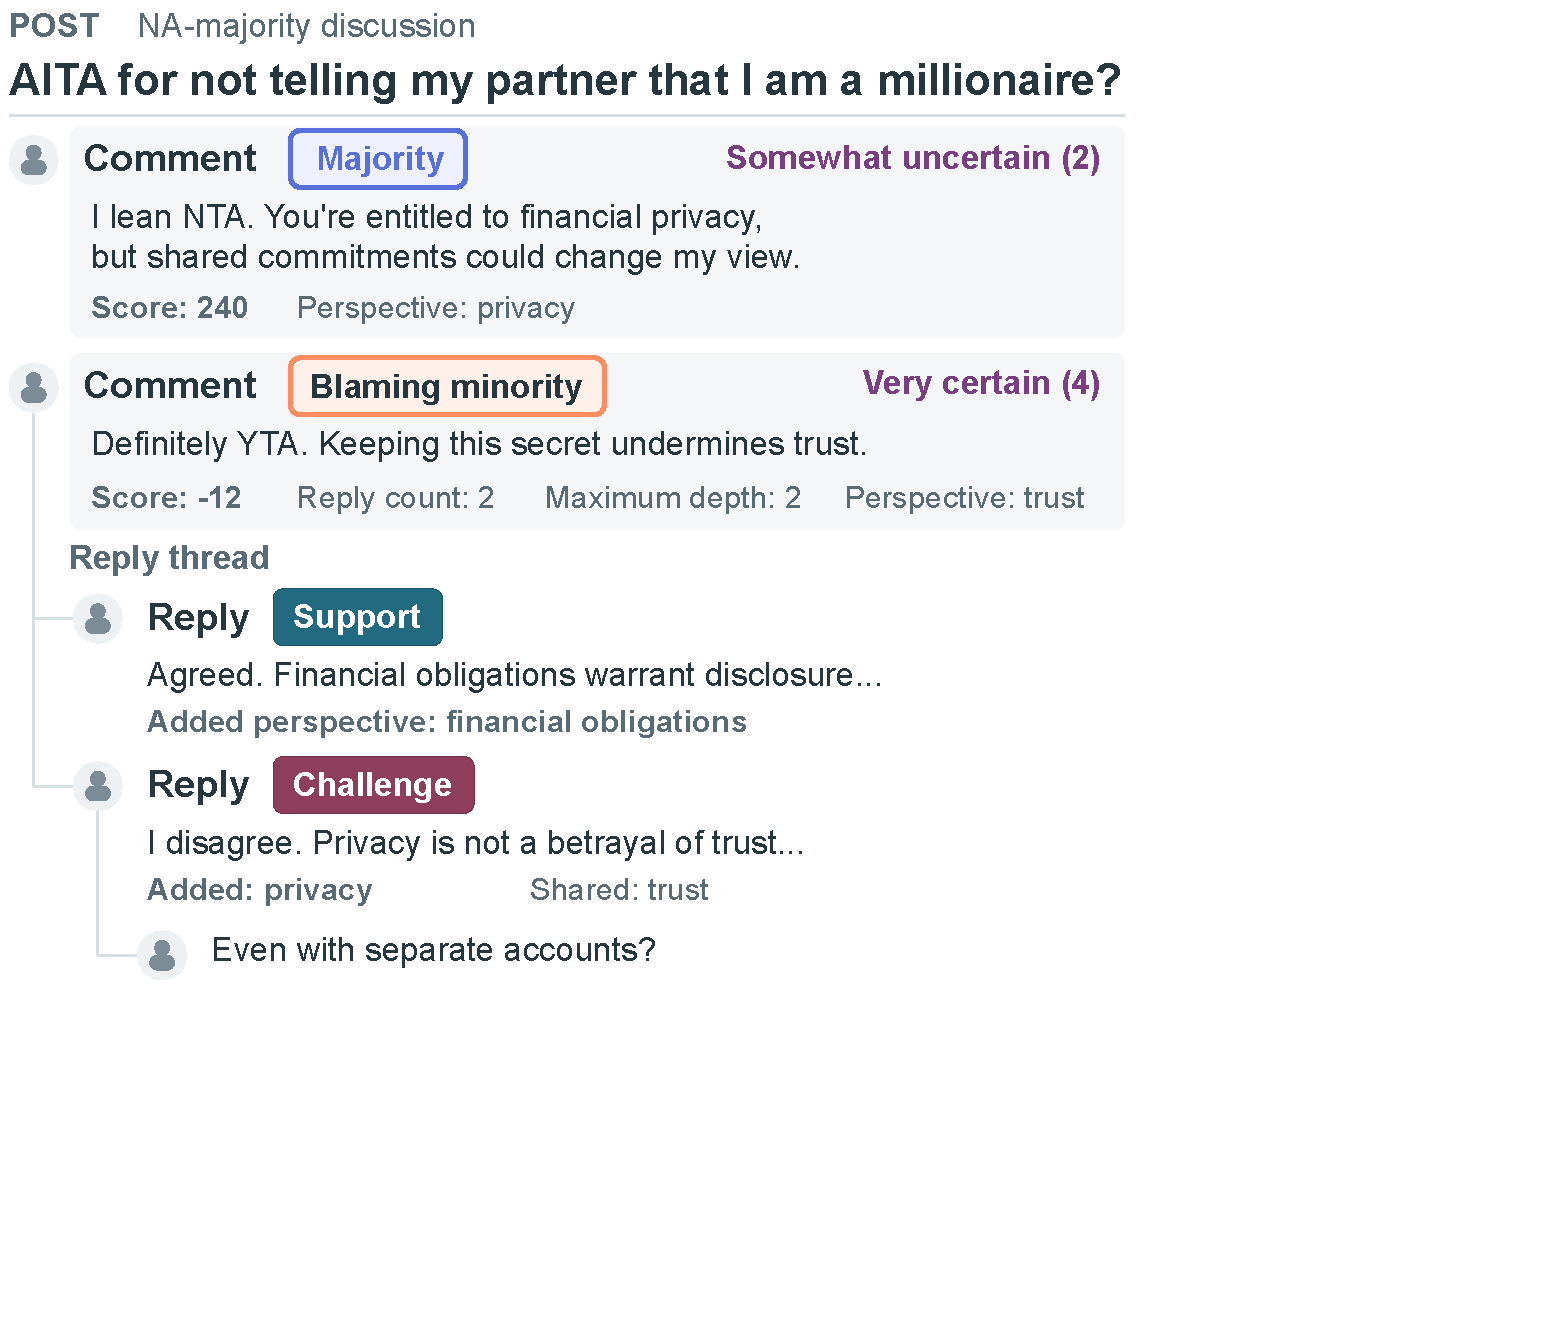
\includegraphics[width=\columnwidth]{figures/fig1_reddit.pdf}
  \caption{Illustrative AITA discussion linking structure, measures, and
  annotations. The blaming comment has two replies and maximum depth two.
  Added/shared perspectives are relative to the comment receiving each reply.
  The title is adapted; text, scores, and labels are schematic, not empirical results.}
  \label{fig:study-overview}
  \Description{An illustrative NA-majority discussion shows a somewhat
  uncertain majority comment and a very certain blaming minority comment.
  The latter has score minus twelve, two replies, and maximum reply depth two.
  A supporting reply adds financial obligations; a challenging reply adds
  privacy while sharing the comment's trust perspective. A further nested
  response illustrates depth two. All comments, scores, and labels are schematic.}
\end{figure}
